\section{Motor measurements}
\label{motorMeasReport}
The purpose of these measurements is to determine the motor parameters. These parameters are:
\begin{itemize}
\item Motor resistance, $R_a$
\item Motor inductance, $L_a$
\item Generator konstant, $K_e$
\item Motor \& wheel friction, $B$
\item Motor \& wheel moment of inertia, $J$
\end{itemize} 

These parameters can be seen in the electromechanical equivalent of a DC-motor, see \autoref{fig:motor_electricalAppendix}. Note that the measurements are performed on the motor with the gear and wheel attached, which are seen as a single mechanical system. Thus, all inertias and dampers measured in the following, are the total values of both the motor, gear and wheel. It is known that the gear ration from motor to shaft is $N_{ms}=19$, while the gear ratio from shaft to wheel is $N_{sw}=\frac{25}{90} \approx 0.2778$

\begin{figure}[H]
\centering
\begin{circuitikz}[american voltages]

	% electrical equivalent circuit
	\draw (0,0) to[V, v^=$V_a$] (0,3);
	\draw (0,3) to[R, i>^=$I_a$, l=$R_a$] (3,3);
	\draw (3,3) to[L, l=$L_a$] (4,3);

	\draw (4,3) -- (5,3);
	\draw (5,0) to[V, v_=\mbox{$V_e = k_e\omega_m$}] (5,3);
	\draw (0,0) -- (5,0);

\end{circuitikz}
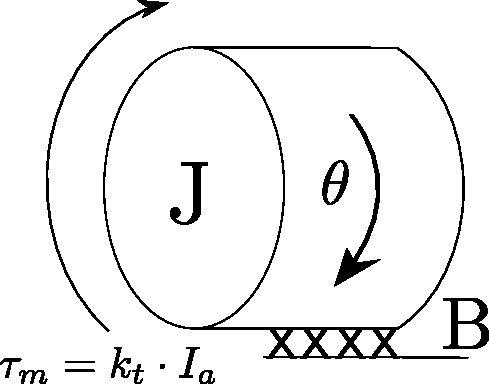
\includegraphics[width=0.25\textwidth]{figures/motorEquivalent.pdf}
\caption{The electromechanical equivalent of a DC motor.}
\label{fig:motor_electricalAppendix}
\end{figure}


\subsubsection{Equipment}
For these measurements, the following equipments are used:
\begin{table}[H]
\centering
\scalebox{0.85}{
\begin{tabular}{|l|l|l|}
\hline\textbf{Name}  & \textbf{AAU No.} & \textbf{Type} \\\hline
HAMEG HM7042-3 & AAU60774         & Power supply        \\\hline
Fluke 37       & AAU33019         & Multimeter          \\\hline 
Fluke I30S	   & AAU78550		  & Amp-meter 			\\\hline
Agilent DSO6034A & AAU64572       & Oscilloscope		\\\hline
-				& AAU08246        &Analog Tachometer    \\\hline
Compact A2108   & AAU77087        &Tachometer    		\\\hline
\end{tabular}
}
\caption{Equipment used to determine motor parameters.}
\label{motor_equipment}
\end{table}


\subsection{Motor resistance, $R_a$}
\subsubsection{Setup}
The rotor is fixed, so the velocity is 0. In steady state, the motor
current and the motor voltage are measured for current from 0 A to 0,9 A.
The voltage is measured with a Fluke 37 (AAU33019) multimeter, and the current is measured using the power supply. The current was tried to be measured using a Fluke 37, but the series resistance in the Fluke might have affected the measurements too much, since the results seen were not realistic. Therefore, the multimeter measuring the current was removed. The current was measured with the power supply after verifying, that the measurements were consistent with the Fluke.

\subsubsection{Results}
\begin{table}[H]
\centering
\scalebox{0.90}{
\begin{tabular}{|l|l|l|}
\hline
\textbf{Current [A]} & \textbf{Voltage [V]}  & \textbf{Resistance [$\Omega$]} \\\hline
0.00             & 0.00              & -                   \\\hline
0.046            & 0.493             & 10.7                \\\hline
0.10             & 0.981             & 9.81                \\\hline
0.20             & 1.518             & 7.59                \\\hline
0.30             & 2.00              & 6.93                \\\hline
0.35             & 2.50              & 7.15                \\\hline
0.47             & 3.06              & 6.52                \\\hline
0.52             & 3.52              & 6.77                \\\hline
0.61             & 4.05              & 6.64                \\\hline
0.68             & 4.54              & 6.68                \\\hline
0.75             & 5.07              & 6.76                \\\hline
0.82             & 5.50              & 6.75                \\\hline
0.91             & 6.02              & 6.65                \\\hline
                 & \textbf{Average:} & \textbf{6.76}	   \\\hline      
\end{tabular}
}
\caption{Results from the resistance measurement.}
\label{resistance_results}
\end{table}
\vspace{-5mm}
\autoref{resistance_results} and \autoref{fig:motorResistance} show that the resistance goes towards linearity at higher currents. The fit for the trend line is $R^2=0.9956$, which means the trend line fits well. From linear regression the resistance is $6.74 \Omega$.

\begin{figure}[H]
	\centering
	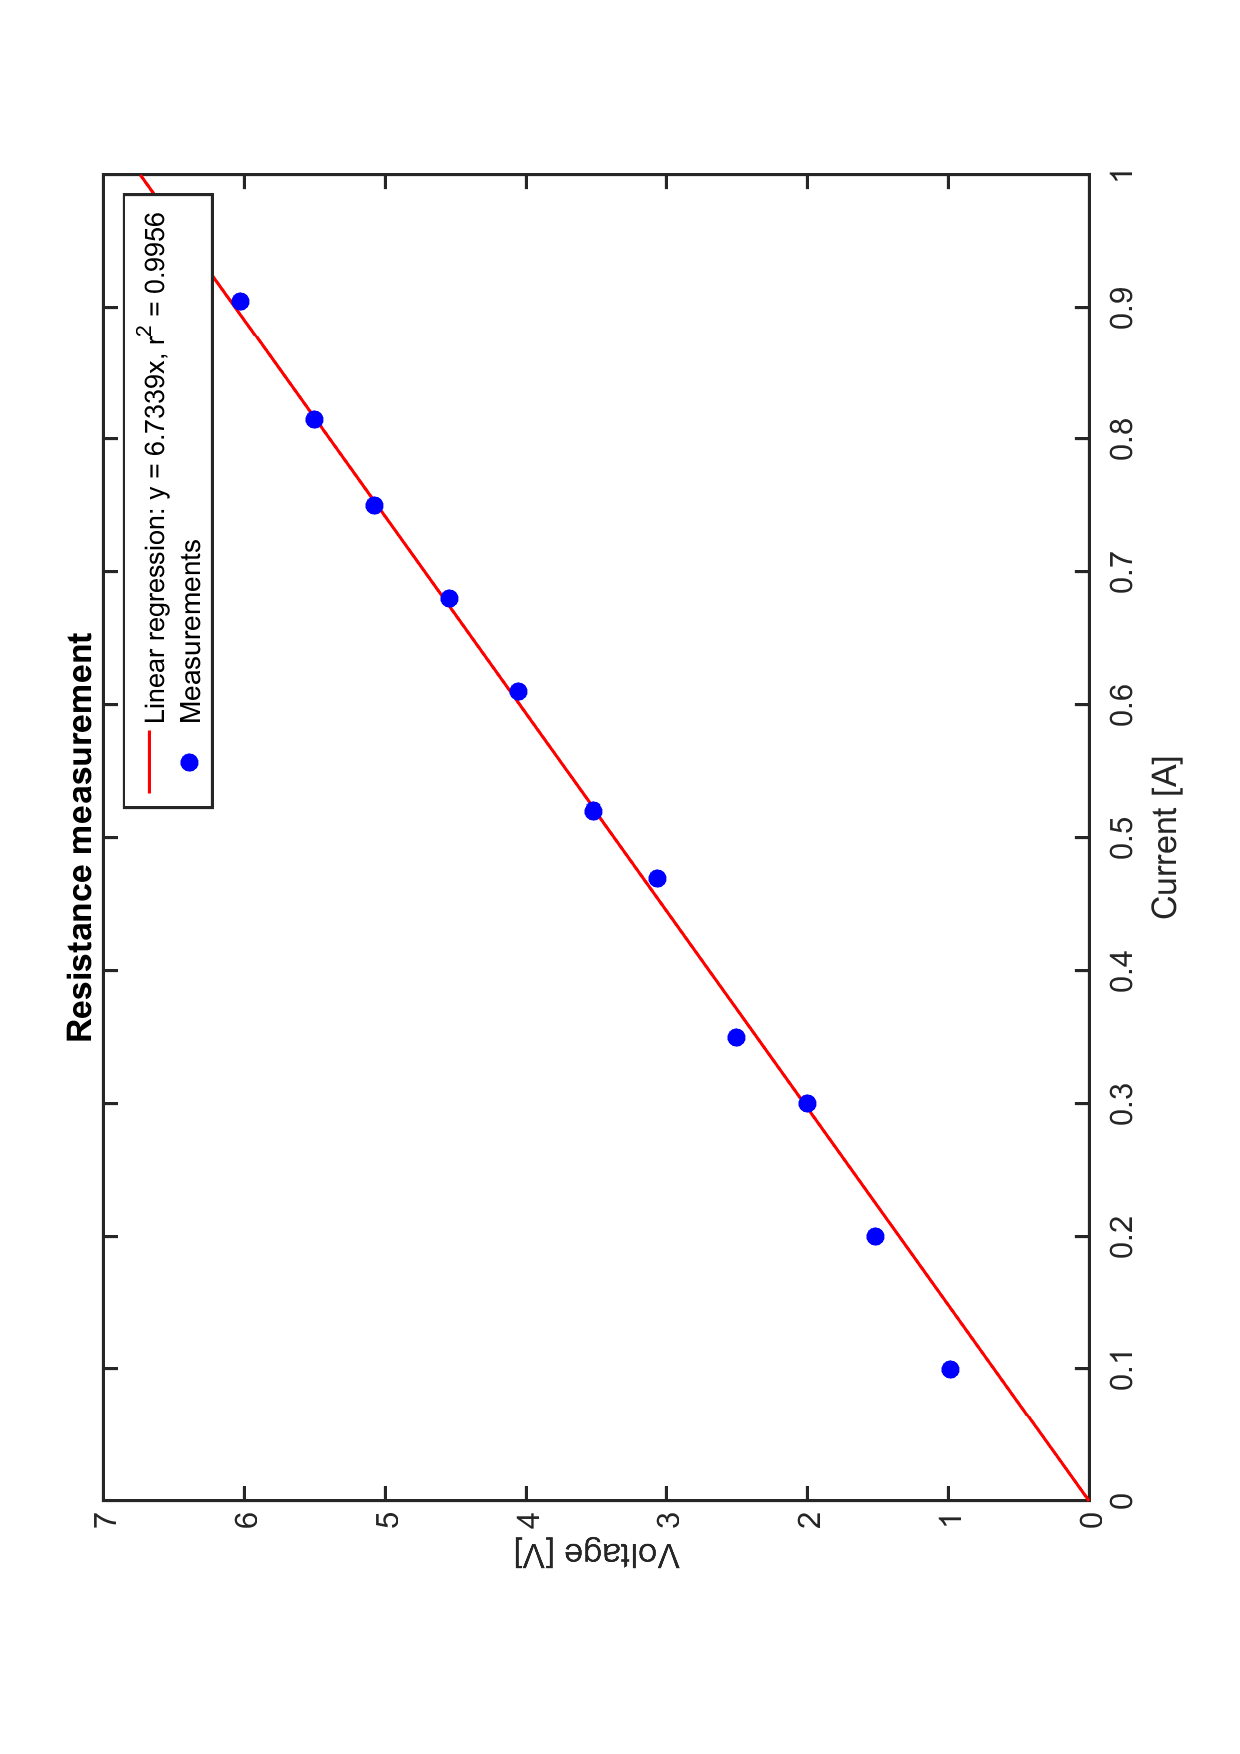
\includegraphics[height=1\textwidth, angle = -90]{figures/motorMeasurements/resistance.pdf}
	\caption{Linear regression of voltage-current measurements to determine the resistance.}
	\label{fig:motorResistance}
\end{figure}

The reason why the measurements are done in steady state is because in steady state, the model of the motor only consist of a resistor. The inductor and voltage generator are short circuited, making it easy to estimate the resistance.

\newpage
\subsection{Motor inductance, $L_a$}
\subsubsection{Setup}
The rotor is fixed so the velocity is 0. The current response
to a voltage input step is measured.
The amp-meter is connected to the oscilloscope, so the current can be measured precisely over time. A voltage step is applied by the PWM drivers with a duty cycle at 200 out of 255.

\subsubsection{Results}
The current plotted as a function of time can be seen in \autoref{fig:motorInductance}. 
\begin{figure}[H]
	\centering
	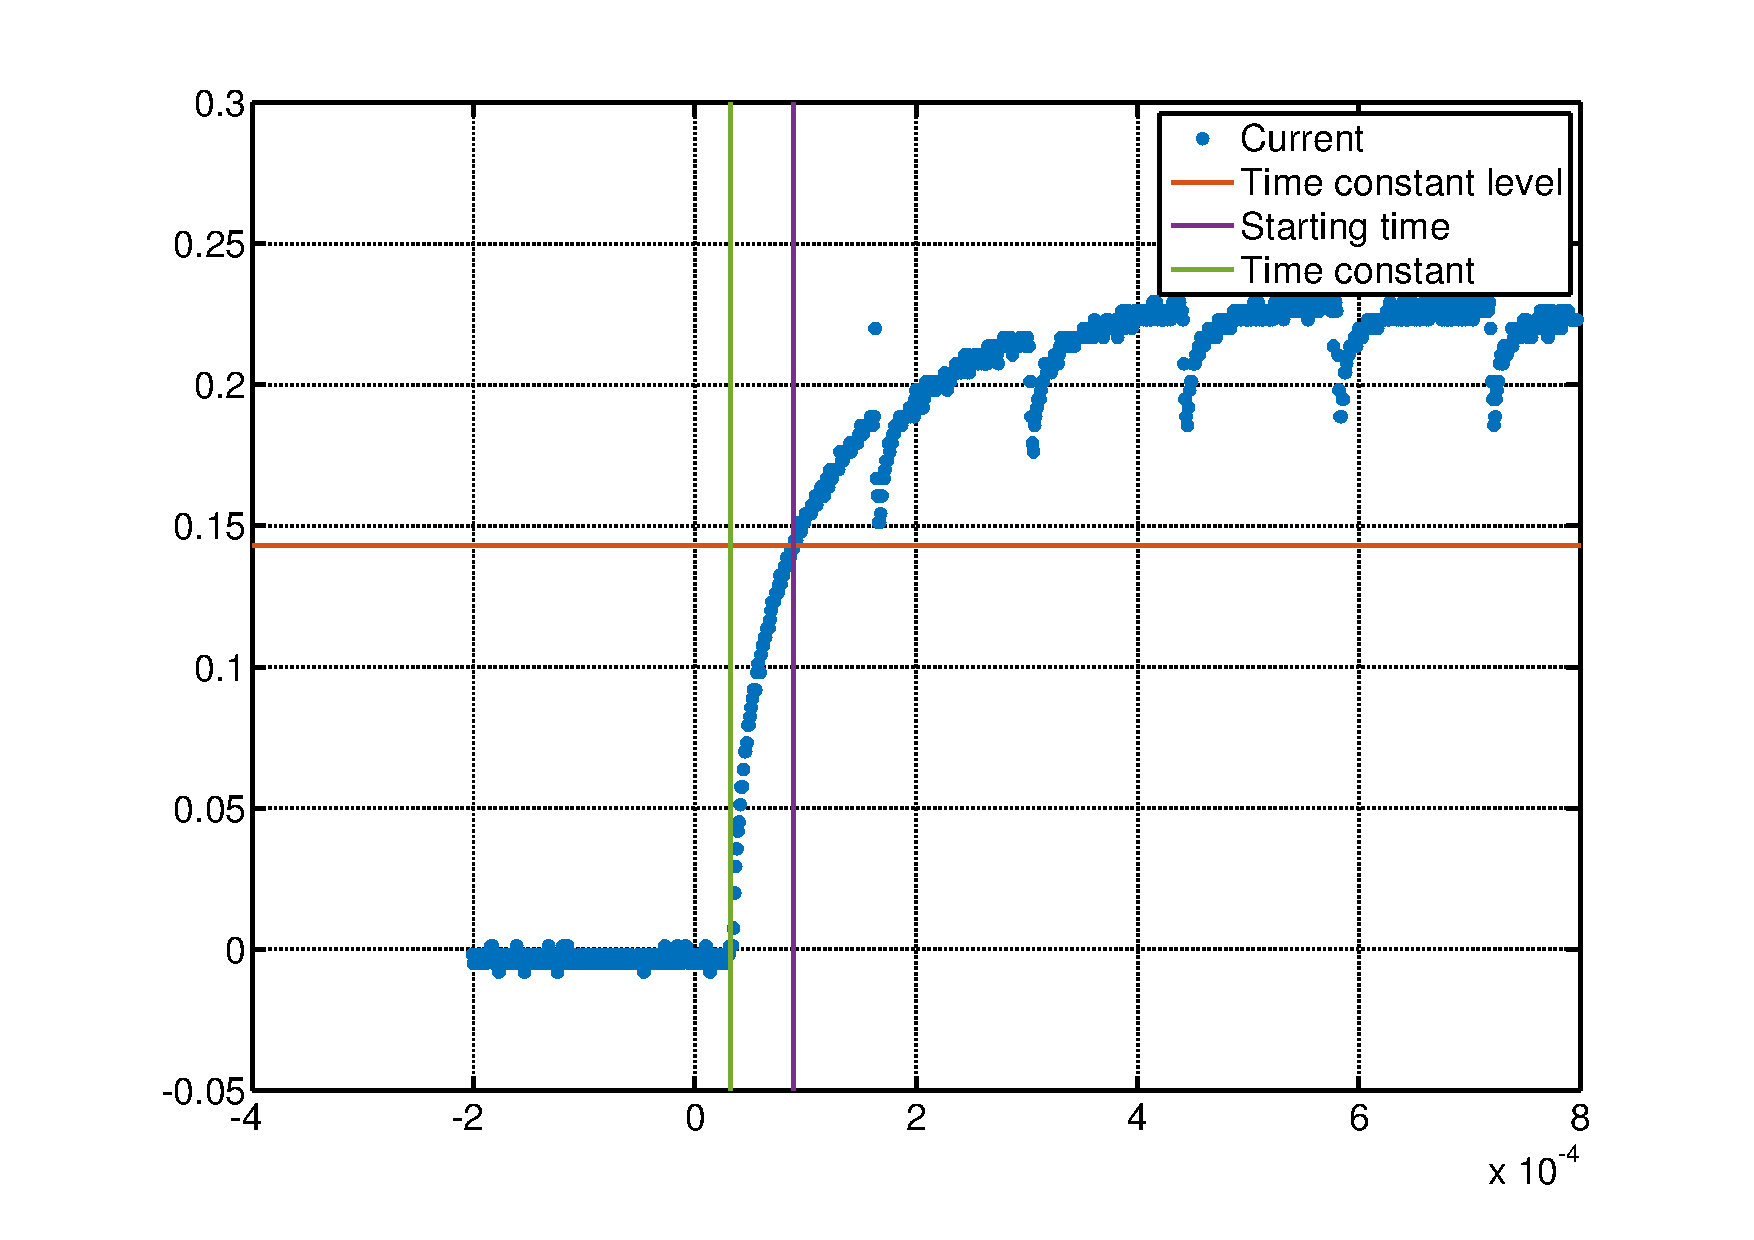
\includegraphics[width=0.95\textwidth]{figures/motorMeasurements/inductance.pdf}
	\caption{Plot of motor current as a function of time, used to find motor inductance.}
	\label{fig:motorInductance}
\end{figure}
The transfer function is of 1st order, because there is only one inductor and no capacitors in the motor equivalent circuit.
The inductance is found using the time constant of a 1st order circuit. It is known that the time constant can be found as $\tau = \frac{L}{R}$, where $I(\tau) = 0.632 \cdot (I_{max} - I_{min})$.
This can be seen in \autoref{fig:motorInductance} as the red line. It is estimated that the voltage step started at the green line. Using this, the time constant is found to be $\tau \approx 57 \, \mu s$.
Thus, the inductance is found:
$$L = R \cdot \tau = 6.74 \, \Omega \cdot 57 \, \mu s = 0.384 \, \text{mH}$$
The inductance is 0.363 mH according to the datasheet, see \citep{maxon}.

\clearpage
\subsection{Generator constant, $K_e$}
\subsubsection{Setup}
In a number of steady state points, the motors voltage and the wheels velocity is measured, using the Fluke multimeter and the onboard encoders. A motor is attached to flexible shaft and to a secondary motor. The motor is fastened using a mounting arm then a current is applied to the secondary motor to make it turn. 

\subsubsection{Results}
The results from the test can be seen in \autoref{ke_results}. In the table, the conversion from velocity $v$ to angular velocity, $\omega_w$, are found as: 
\begin{align}
\omega_w &= \frac{\text{v}}{r_w}\\
\omega_m &= \frac{1}{N_{ms}}\cdot\frac{1}{N_{sw}}\cdot\omega_w
\end{align}
\begin{where}
	\va{$\omega_w$}{is the angular velocity of the wheel}{rad/s}
	\va{$v$}{is the translatoric velocity of the wheel}{m/s}
	\va{$r_w$}{is the radius of the wheel}{m}
	\va{$\omega_m$}{is the angular velocity of the motor}{rad/s}
	\va{$N_{ms}$}{is the gearing ratio from the motor to the shaft}{1}
	\va{$N_{sw}$}{is the gearing ratio from the shaft to the wheel}{1}
\end{where}
 
Also, $K_e$ can be found using the expression $K_e = \frac{U_a}{\omega}$.
Note that the measured velocity has been divided with the gear ratios ($N_{ms} = \frac{1}{19} \approx 0.053$ and $N_{sw} = \frac{25}{90} \approx 0.277$), to obtain the angular velocity of the motor instead of the wheel, as it is the motors angular velocity, $\omega_m$ that is used.


\begin{table}[H]
\centering
\scalebox{1}{
\begin{tabular}{|l|l|l|l|l|}
\hline
\textbf{$\mathbf{speed_{w}}$} \textbf{[m/s] }& $\boldsymbol{\omega_w }$ \textbf{[rad/s]}& $\boldsymbol{\omega_m }$ \textbf{[rad/s]} & \textbf{Voltage [V]} & $\boldsymbol{K_e [\text{V}/\frac{\text{rad}}{\text{s}}]}$ \\ \hline
0.34       & 5.81      & 397.5      & 4.25     & 0.0107   \\ \hline
0.74       & 12.65     & 865.2      & 9.15     & 0.0106   \\ \hline
0.46       & 7.86      & 537.8      & 5.70     & 0.0106   \\ \hline
0.33       & 5.64      & 385.8      & 4.00     & 0.0104   \\ \hline
0.22       & 3.76      & 257.2      & 2.70     & 0.0105   \\ \hline
\end{tabular}
}
\caption{Results from the test to determine the $K_e$ factor.}
\label{ke_results}
\end{table}
Averaging the results in \autoref{ke_results}, the $K_e$ factor is determined to be:
$$K_e = 10.5 \frac{\text{mV}}{\frac{\text{rad}}{s}}$$

\subsection{Motor \& wheel friction, B}
\subsubsection{Setup}
In a number a steady state points, the motor current and motor velocity is measured. This is done using the ampmeter and the encoders.

\subsubsection{Results}
In steady state, i.e. constant angular velocity, the friction torque is $\tau_B = K_t \cdot i_a$.
This is true since the resultant torque is 0 when the system is in steady state. Thus, all torque applied by the motor must be countered by an equal torque in opposite direction due to friction.

In \autoref{friction_raw_results} measurements of the angular velocity and the motor current $i_a$ are listed.
\begin{table}[H]
\centering
\scalebox{0.85}{
\begin{tabular}{|l|l|}
\hline \textbf{$\omega_m$ [$\text{rad}/\text{s}$]} & $\mathbf{i_a [A]}$ \\\hline
1216.00	& 0.083  \\\hline
1099.08	& 0.080  \\\hline
841.85	& 0.073  \\\hline
502.77	& 0.066  \\\hline
362.46	& 0.092  \\\hline
748.31	& 0.096  \\\hline
1052.31	& 0.100  \\\hline
1180.92	& 0.106  \\\hline
\end{tabular}
}
\caption{The measurements of the angular velocity and $I_a$ for determining the damper coefficient B.}
\label{friction_raw_results}
\end{table}

The motor torque, and thus the damper torque $\tau_B$, can be found using $\tau_B = K_t \cdot i_a$, where $K_t = K_e =  10.5 \frac{ \text{mNm}}{A}$ 

Since it is known that the resultant torque of a damper can be found as $\tau_B = B\cdot \omega$, B can be found since both $\tau_B$ and $\omega$ are known. The results can be seen in \autoref{friction_calculated}.

\begin{table}[H]
\centering
\scalebox{0.90}{
\begin{tabular}{|l|l|l|}
\hline
$\boldsymbol{\omega_m [\frac{rad}{s}]}$ & $\boldsymbol{\tau_B [Nm]}$ & \textbf{B} $[\frac{\text{Nm}}{\frac{\text{rad}}{s}}]$ \\ \hline
1216,00	& $875,27\cdot 10^{-6}$		& $0,720\cdot 10^{-6}$   \\ \hline
1099,08	& $843,63\cdot 10^{-6}$		& $0,768\cdot 10^{-6}$   \\ \hline
841,85	& $769,82\cdot 10^{-6}$		& $0,914\cdot 10^{-6}$   \\ \hline
502,77	& $696,00\cdot 10^{-6}$		& $1,384\cdot 10^{-6}$   \\ \hline
362,46	& $970,18\cdot 10^{-6}$		& $2,677\cdot 10^{-6}$   \\ \hline
748,31	& $1012,36\cdot 10^{-6}$	& $1,353\cdot 10^{-6}$   \\ \hline
1052,31	& $1054,54\cdot 10^{-6}$	& $1,002\cdot 10^{-6}$   \\ \hline
1180,92	& $1117,81\cdot 10^{-6}$	& $0,947\cdot 10^{-6}$   \\ \hline
\end{tabular}
}
\caption{The friction torque and friction coefficient B.}
\label{friction_calculated}
\end{table}
\vspace{-5mm}
Averaging the results for B in \autoref{friction_calculated}, B is found as:
$$B=1.22 \frac{\mu\text{Nm}}{\frac{\text{rad}}{s}}$$


\subsection{Coulomb friction, $\tau_c$} \label{app:coloumbTest}
\subsubsection{Setup}
In a number a steady state points, the motor current and applied voltage are measured. The voltage is applied by the Hameg power supply, the current is measured with the amp-meter, and the voltage with the multimeter. Then steps are made on the Hameg with approximately 0.1 V until 2.4 V from there the steps are 0.2 V to 5 V.  

\subsubsection{Results}
It is expected that the current can be estimated by two straight lines, because of the coulomb friction. Until $Ia \cdot k_t$ equals the coulomb friction. The current is expected to have a steep slope, and when the motor starts rotating, the slope is expected to be less steep. This can be seen in \autoref{fig:coloumb_friction}, where these slopes and offsets have been estimated using curve fitting. 

\begin{figure}[H]
	\centering
	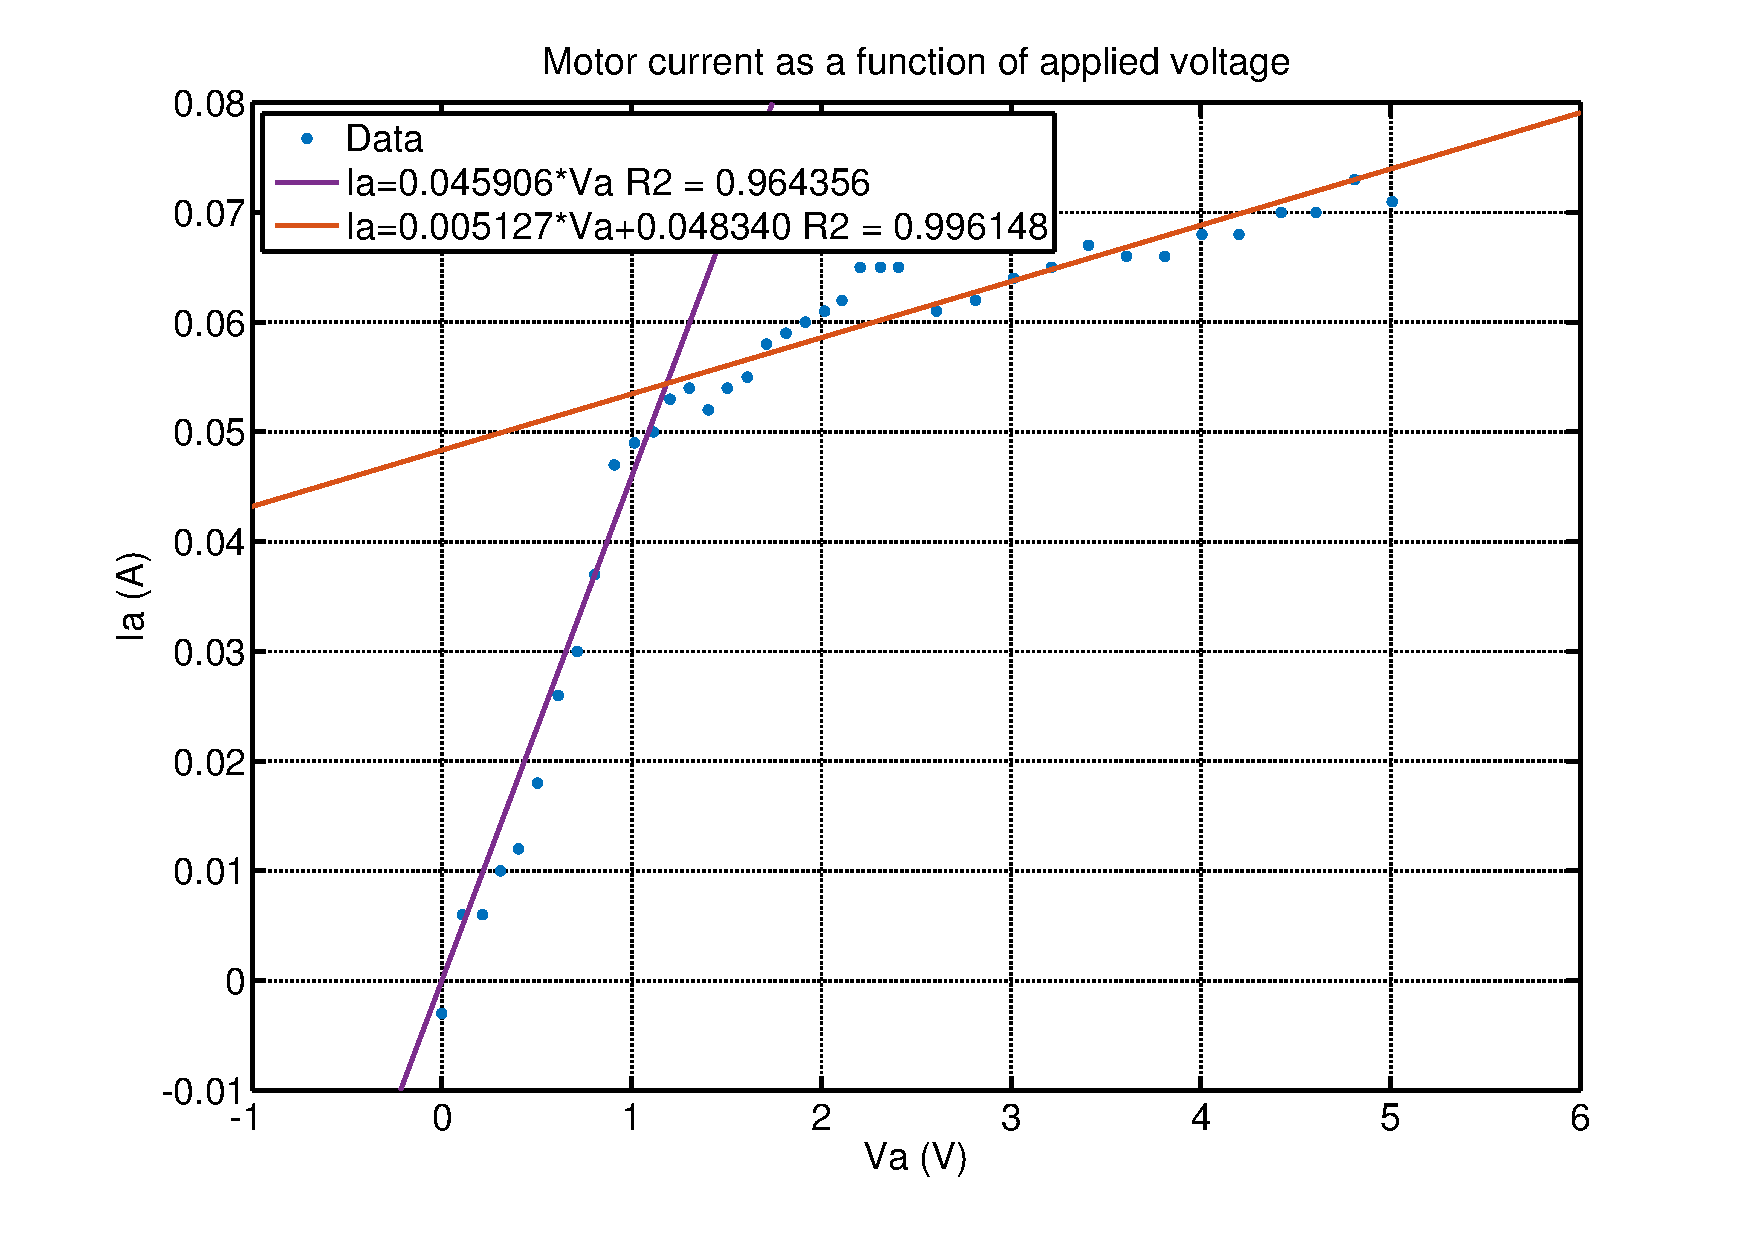
\includegraphics[width=\textwidth]{figures/motorMeasurements/coloumb_friction.pdf}
	\caption{Motor current as a function of applied voltage with two curves fitted to the data area before and after wheel started turning.}
	\label{fig:coloumb_friction}
\end{figure}

The coulomb friction can be found based in \autoref{fig:coloumb_friction} by finding the current in the intersection between the two lines and then multiplying with $k_t$.

\begin{align}
	0.045906 \cdot Va&=0.005127 \cdot Va+0.048340\\
	Va&=1.18541 \, \text{V}
\end{align}
The current in the intersection can be found by inserting $Va$ in any of the equations.
\begin{align}
	Ia=0.045906 \cdot 1.18541\\
	Ia=0.054417 \, \text{A}
\end{align}

The coulomb friction can then be found as:
\begin{align}
	\tau_c &= Ia \cdot k_t\\
	\tau_c &= 0.054417 \, \text{A} \cdot 0.0105 \frac{\text{Nm}}{\text{A}}\\
	\tau_c &= 571.4 \mu \text{Nm}
\end{align}

Note that during another version of this test, the maximum velocity was found to be 1.17 m/s when driven by the segway's PWM signal. 

\subsection{Moment of inertia, J}
\subsubsection{Setup}
The motor is rotated with a fixed velocity, after which the motor is turned off i.e., making $i_a = 0$ by setting the duty cycle to 0. The motor velocity is measured with a interval of 5 ms. This is done by using the onboard encoders and a timer interrupt.

\subsubsection{Results}
Looking at a motor's kinematics, the mechanical equation can be expressed as shown in \autoref{eq:motorkinematic} 
\begin{equation}\label{eq:motorkinematic}
I \cdot \dot \omega(t) = k_t \cdot Ia(t)- B \cdot \omega(t)- \tau_c
\end{equation}

If it is assumed that the motor is running at $\omega(0)$ and the motor then is terminated $(Ia = 0)$, the differential equation can then be solved. The result can be seen in \autoref{eq:motorkinematic2}

\begin{equation}\label{eq:motorkinematic2}
\omega(t) = -\frac{\tau_c}{B} + \left(\omega(0)+\frac{\tau_c}{B}\right) \cdot e^{-\frac{B}{I} \cdot t}
\end{equation}

By knowing this, the output graph seen in \autoref{fig:motorInertia}, shows that the rotational speed as a function of time can be interpreted. By inserting the previous found values, a fit has to be found manually, this is the purple graph in \autoref{fig:motorInertia}. A better fit can be found if the damper is divided by 8 before fitting the inertia. This can be seen as the orange graph in \autoref{fig:motorInertia}.

\begin{figure}[H]
	\centering
	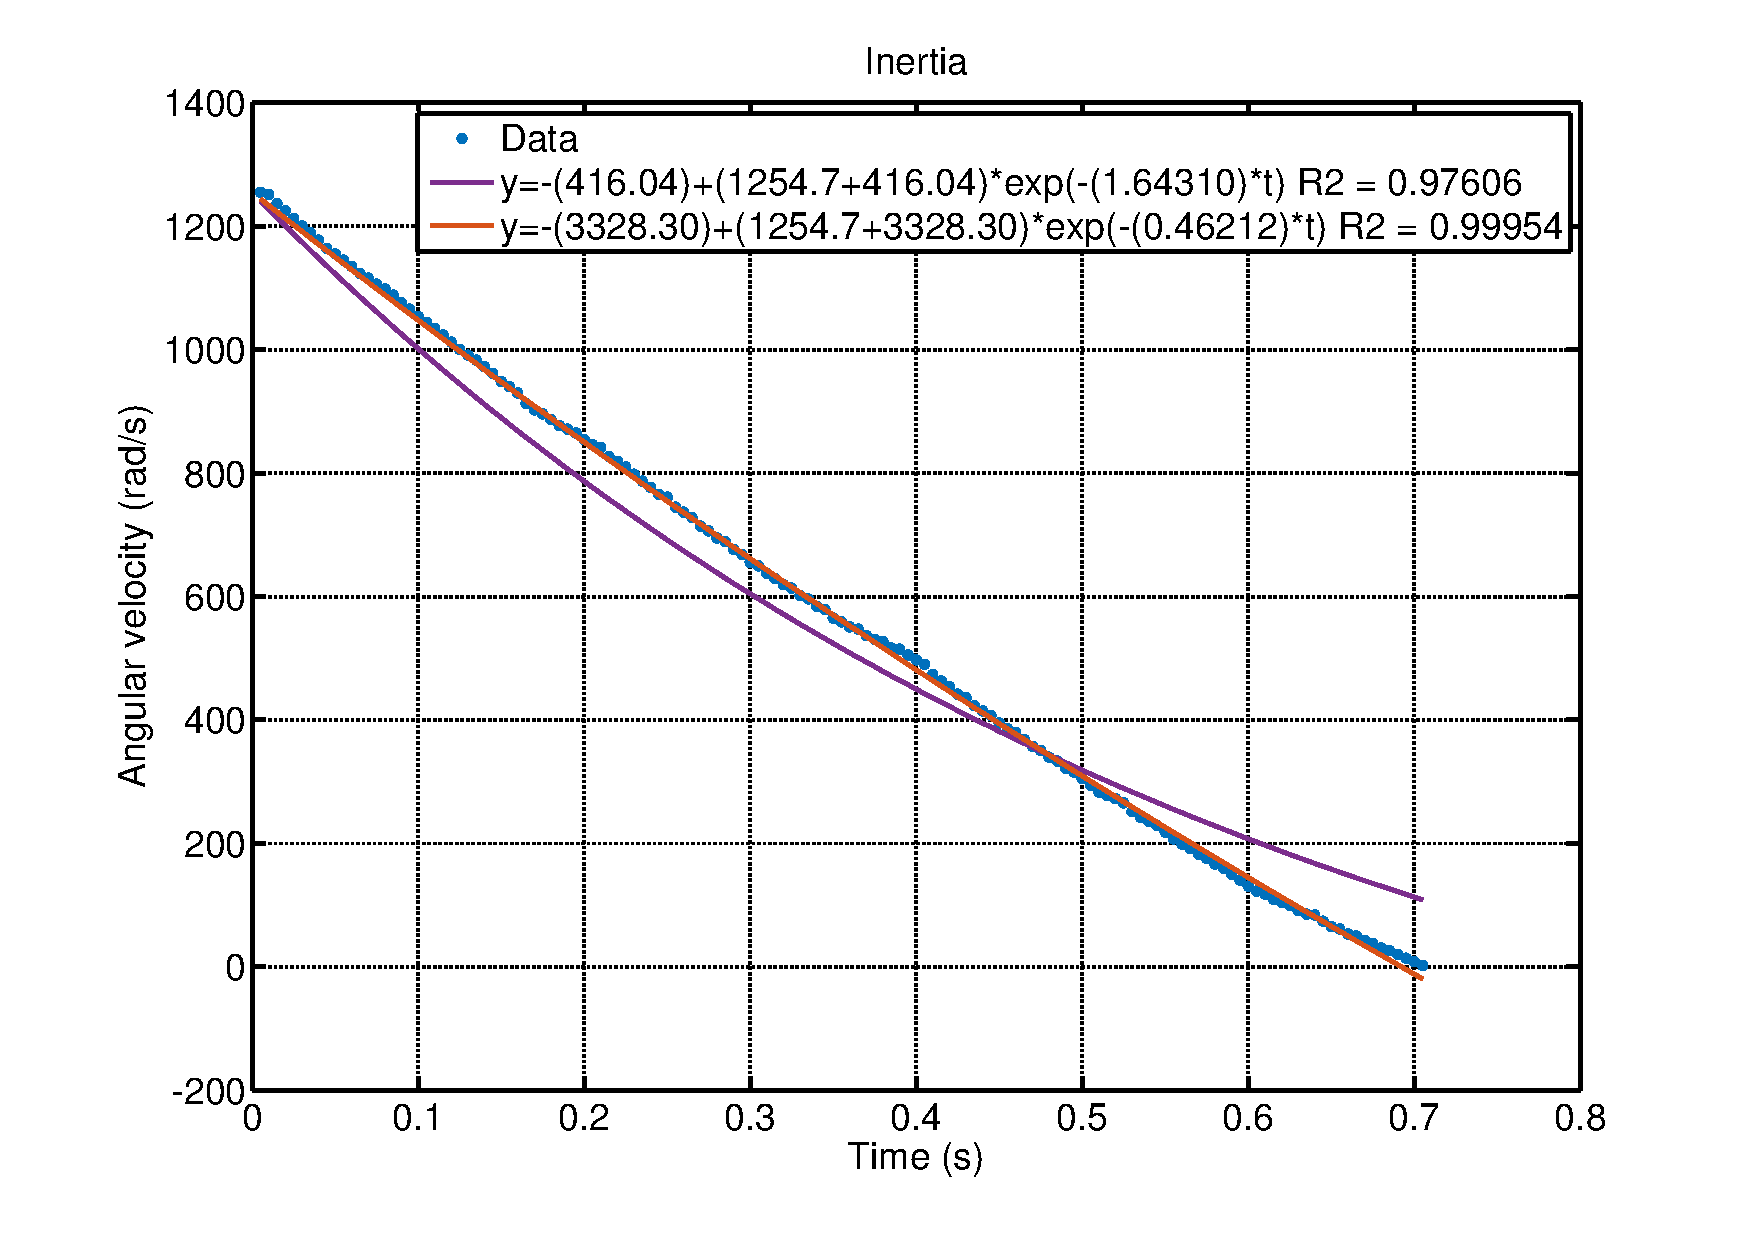
\includegraphics[width=0.90\textwidth]{figures/motorMeasurements/inertia.pdf}
	\caption{Motor velocity as a function of time, when the motor current $i_a$ is set to 0 at time 0.}
	\label{fig:motorInertia}
\end{figure}

Because of this measurement, it is decided to divide the damper by a factor of 8 in the model. Based on this, the damper and inertia is found and can be seen in \autoref{tab:inertia}

\begin{table}[H]
\centering
\scalebox{0.90}{
\begin{tabular}{|l|l|}
\hline
Damper	& $152.5 \cdot 10^{-9} \frac{\text{sNm}}{\text{rad}} $	 \\ \hline
Inertia	& $330 \cdot 10^{-9} \frac{kg}{m^2}$	 \\ \hline
\end{tabular}
}
\caption{The friction coefficient B, and Inertia J, to be used in model.}
\label{tab:inertia}
\end{table}


%\subsection{Calculation of moment of inertia}
%In order to calculate the moment of inertia of the whole motor and wheel system, all the parts must be taken into account. it is thus 3 inertias that are to be found:
%The inertia of the motor, $J_m$, the shaft, $J_s$ and the wheel $J_w$.
%The shaft inertia is comprised of two inertias - that of the gear attached to the motor, $J_{g}$, see {subsec:motors} and the small inner gear on the wheel, $J_{gi}$, see {subsec:wheels}. Since the two inertias are placed on the same axis of rotation, they can simply be summed to obtain the total inertia. This is because the inertia is defined as:
%\begin{equation}
%J = \sum_{i = 1}^{N}m_i r_i^2
%\end{equation}
%
%\begin{where}
%\va{J}{is the moment of inertia}{kg$\text{m}^2$}
%\va{m}{is the i'th point mass}{kg}
%\va{r}{is the distance to the i'th point mass from the center of rotation}{$\text{m}^2$}
%\end{where}
%
%Thus, if two inertias are put together, and they have the same point of rotation, they can be summed to get the total inertia, as it would be equal to summing all the point masses of the total system.
%
%Since the motor cannot be taken apart, the inertia of the motor and motor gear cannot be determined accurately, but only estimated. However, instead of doing a rough estimation of these inertias, the inertias from the datasheet are found.
%
%The inertias of the inner and outer gear on the wheel, named $J_{gi}$ and $J_{go}$, have to be calculated. The parts of the wheel identified as the inner gear and the outer gear will be treated as hollow cylinders in the calculations presented below.
%
%Let $J$ be the moment of inertia of a hollow cylinder with $\rho$ its density, $m$ its mass, $h$ its height, $R$ its radius and $e$ its thickness as can be seen on \autoref{fig:HollowCylinder}.
%
%\begin{figure}[H]
%	\centering
%	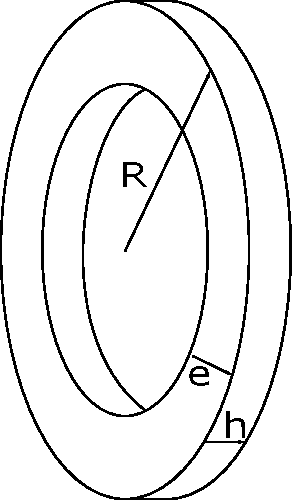
\includegraphics[width=0.2\textwidth]{figures/motorMeasurements/hollow_cylinder.pdf}
%	\caption{Figure representing a hollow cylinder and the values that are associated with it}
%	\label{fig:HollowCylinder}
%\end{figure}
%
%
%The definition of the moment of inertia is $J = \int_{V}^{} r^2 dm$ \citep{Iner} with $dm = \rho dV$ the mass element, $dV = dr d\theta r  dz$ being the volume element. Hence the following equation: 
%\begin{align*}
%J &= \int_{V}^{} r^2 dm \\
%&= \rho \int_{V}^{} r^2 dV \\
%&= \rho \int_{0}^{h} \int_{0}^{2 \pi} \int_{R-e}^{R} r^2 dr d\theta r dz \\
%&= \rho \int_{0}^{h} \int_{0}^{2 \pi} \frac{R^4 - (R-e)^4}{4} d\theta dz \\
%&= \rho \int_{0}^{h} \frac{R^4 - (R-e)^4}{4} 2 \pi dz \\
%&= \rho \frac{R^4 - (R-e)^4}{2} \pi h
%\end{align*}
%
%The density $\rho$ is unknown, however, the mass $m$ can be measured as well as the different lengths $R$ and $e$ as can be seen on \autoref{fig:HollowCylinder}, thereby the equation above should be solely depending upon the previously mentioned  values.
%
%Since $m = [kg]$ and $\rho = [\text{kg} \cdot \text{m}^{-3}]$, it is possible to establish the following relation: $\text{kg} = (\text{kg} \cdot \text{m}^{-3}) \cdot \text{(m)} \cdot \text{(m)}^2$ since the mass is equal to the density times the volume, which corresponds to $m = \rho \pi h (R^2-(R-e)^2)$.
%
%As a result, the inertia can be written as follows
%\begin{align*}
%J &= \rho \frac{R^4 - (R-e)^4}{2} \pi h \\
%&= (\rho \pi h (R^2-(R-e)^2)) \cdot (\frac{1}{2} (R^2+(R-e)^2)) \\
%&= m \frac{1}{2} (R^2+(R-e)^2)
%\end{align*}
%
%\begin{table}[H]
%\centering
%\begin{tabular}{lllll}
%\cline{1-4}
%\multicolumn{1}{|l|}{\textbf{}}           & \multicolumn{1}{l|}{\textbf{Mass}}           & \multicolumn{1}{l|}{\textbf{Outer radius}}     & \multicolumn{1}{l|}{\textbf{Inner radius}}            &  \\ \cline{1-4}
%\multicolumn{1}{|l|}{\textbf{Inner gear}} & \multicolumn{1}{l|}{$m_{gi} = 19 \text{g}$}  & \multicolumn{1}{l|}{$R_{gi} = 1,35 \text{cm}$} & \multicolumn{1}{l|}{$R_{gi}-e_{gi} = 0,25 \text{cm}$} &  \\ \cline{1-4}
%\multicolumn{1}{|l|}{\textbf{Outer gear}} & \multicolumn{1}{l|}{$m_{go} = 133 \text{g}$} & \multicolumn{1}{l|}{$R_{go} = 5,95 \text{cm}$} & \multicolumn{1}{l|}{$R_{go}-e_{go} = 4,55 \text{cm}$} &  \\ \cline{1-4}
%                                          &                                              &                                                &                                                       & 
%\end{tabular}
%\caption{Measured values on both wheels of the gear}
%\label{GearMeasurements}
%\end{table}
%
%Inserting these values in the fomulas, the calculated values of $J_{gi}$ and $J_{go}$ are:
%\begin{align*}
%J_{gi} &= \frac{1}{2} m_{gi} (R_{gi}^2+(R_{gi}-e_{gi})^2)\\
%&= 0.5 \cdot 0.019 (0.0135^2+0.0025^2) \\
%&= 1.79 \cdot 10^{-6} \text{kg} \cdot \text{m}^2 \\\\
%J_{go} &= \frac{1}{2} m_{go} (R_{go}^2+(R_{go}-e_{go})^2)\\
%&= 0,5 \cdot 0.133 (0.0595^2+0.0455^2) \\
%&= 37.3 \cdot 10^{-3} \text{kg} \cdot \text{m}^2
%\end{align*}
%
%From the datasheet of the motor \citep{maxon}, the moment of inertia of the motor rotor, $J_m$, is known:
%\begin{equation}
%J_m = 4.36 \text{g} \cdot \text{cm}^2 = 436 \cdot 10^{-9} \text{kg} \cdot \text{m}^2
%\end{equation}
%
%From the datasheet of the gear \citep{gear}, the moment of inertia of the motor rotor, $J_g$, is known:
%\begin{equation}
%J_{g} = 0.05 \text{g} \cdot \text{cm}^2 = 5 \cdot 10^{-9} \text{kg} \cdot \text{m}^2
%\end{equation}
%
%As described above, the shaft inertia is comprised of the motor gear inertia and inner wheel gear inertia:
%\begin{equation}
%J_{s} = J_{g} + J_{gi} = 5 \cdot 10^{-9} \text{kg} \cdot \text{m}^2 + 1.79 \cdot 10^{-6} \text{kg} \cdot \text{m}^2 \approx 1.8 \cdot 10^{-6} \text{kg} \cdot \text{m}^2
%\end{equation}
%
%The inertia of the wheel is simply the inertia of the outer gear on the wheel, i.e.:
%\begin{equation}
%J_{w} = J_{go} =  37.3 \cdot 10^{-3} \text{kg} \cdot \text{m}^2
%\end{equation}
%
%Thus, all three inertias have been determined. The total inertia for the entire system can be found as defined in \autoref{TotalInertia}:
%
%\begin{equation}
%J_{T} \equiv J_m + N_{ms}^2(J_s + N_{sw}^2 J_w)
%\end{equation}
%
%From \autoref{subsec:wheels}, it is known that $n_s = 25$ and $n_w = 90$, resulting in a gear ratio of:
%$$N_{sw} = \frac{n_m}{n_w} = \frac{25}{90} \approx 0.2778 $$ 
%
%From \citep{gear} the gear ratio from motor to shaft is known:
%\begin{equation}
%N_{ms} = \frac{1}{19} \approx 0.053
%\end{equation}
%
%Inserting the values, the total inertia becomes:
%\begin{equation}
%J_T = 8.53 \cdot 10^{-6} \text{kg} \cdot \text{m}^2
%\end{equation}
